\chapter{Supported Hardware Buses} \label{ch:hw_buses}

Hardware buses implemented in GEX are presented in this chapter. The description of each bus is accompanied by several examples of devices that can be interfaced with it. The reader is advised to consult the official specifications and particular devices' datasheets for additional technical details.

\section{UART and USART} \label{sec:theory-usart}

The \textit{Universal Synchronous / Asynchronous Receiver Transmitter} has a long history and is still in widespread use today. It is the protocol used in RS-232, which was once a common way of connecting modems, printers, mice and other devices to personal computers. UART framing is also used in the industrial bus RS-485.

\begin{figure}
	\centering
	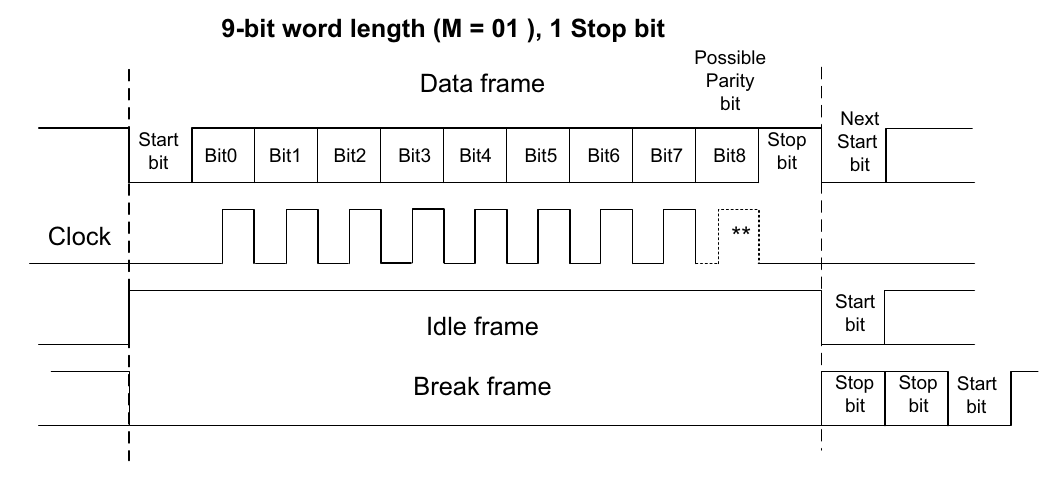
\includegraphics[width=.8\textwidth] {img/usart.png}
	\caption[UART frame structure]{\label{fig:uart-frame}UART frame, as shown by the STM32F072 Reference Manual. Break frames are used by some UART based protocols, like LIN (Local Interconnect Network).}
\end{figure}

UART and USART are two variants of the same interface. USART includes a separate clock signal, while the UART timing relies on a well-known clock speed and the bit clock is synchronized by start bits. USART was historically used in modems to achieve higher bandwidth, but is now mostly obsolete.

USART, as implemented by microcontrollers such as the STM32 family, is a two-wire full duplex interface that uses 3.3\,V or 5\,V logic levels. The data lines are in the high logical level when idle. A frame, pictured in figure \ref{fig:uart-frame} starts by a start-bit (low level for the period of one bit) followed by \textit{n} data bits (typically eight), an optional parity bit and a period of high level called a stop bit or stop bits, usually between one and two bits long.
 
RS-232 uses the UART framing, but its logic levels are different: logical 1 is represented by negative voltages $-3$ to $-25$\,V and logical 0 uses the same range, but positive. To convert between RS232 levels and TTL (5\,V) levels, a level-shifting circuit such as the MAX232 can be used. In RS232, the two data lines (Rx and Tx) are accompanied by RTS (Ready To Send), CTS (Clear To Send) and DTR (Data Terminal Ready) which facilitate handshaking and hardware flow control. In practice, those additional signals are often unused or their function differs; for instance, Arduino boards (using a USB-serial converter) use the DTR line as a reset signal to automatically enter their bootloader for firmware flashing.

\subsection{Examples of Devices Using UART}

\begin{itemize}
	\item \textbf{MH-Z19B} - NDIR CO2 concentration sensor 
	\item \textbf{NEO-M8} - uBlox GPS module
	\item \textbf{ESP8266} with AT firmware - a WiFi module
	\item \textbf{MFRC522} - NFC MIFARE reader/writer IC (also supports other interfaces)
\end{itemize}

\section{SPI} \label{sec:theory-spi}

SPI (Serial Peripheral Interface) is a point-to-point or multi-drop master-slave interface based on shift registers. The SPI connection with multiple slave devices is depicted in figure \ref{fig:spi-multislave}. It uses at least 4 wires: SCK (Serial Clock), MOSI (Master Out Slave In), MISO (Master In Slave Out) and SS (Slave Select). SS is often marked CSB (Chip Select Bar) or NSS (Negated Slave Select) to indicate it's active low. Slave devices are addressed using their Slave Select input while the data connections are shared. A slave that's not addressed releases the MISO line to a high impedance state so it doesn't interfere in ongoing communication.

Transmission and reception on the SPI bus happen simultaneously. A bus master asserts the SS pin of a slave it wishes to address and then sends data on the MOSI line while receiving a response on MISO. It's customary that the slave responds with zeros or a status byte as the first byte of the response.

SPI devices often provide a number of control, configuration and status registers that can be read and written by the bus master. The first byte of a command usually contains one bit that determines if it's a read or write access, and an address field selecting the target register.

\begin{figure}
	\centering
	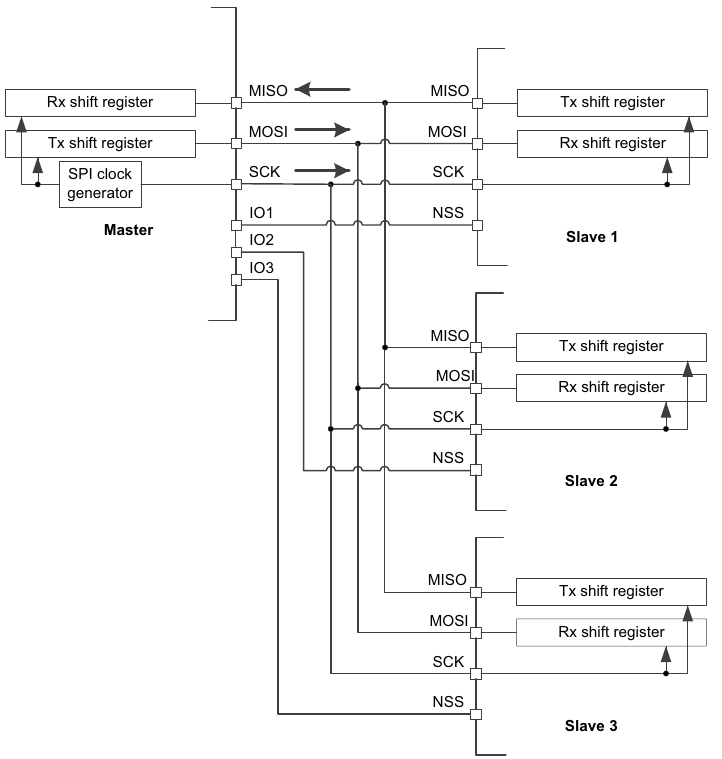
\includegraphics[width=.7\textwidth] {img/spi-multislave.png}
	\caption[SPI master with multiple slaves]{\label{fig:spi-multislave}A SPI bus with 1 master and 3 slaves, each enabled by its own Slave Select signal (\textit{STM32F072 Reference Manual})}
\end{figure}

\subsection{Examples of Devices Using SPI}

\begin{itemize}
	\item \textbf{SX1276} - LoRa transceiver
	\item \textbf{nRF24L01+} - 2.4\,GHz ISM band radio module
	\item \textbf{L3GD20} - 3-axis gyroscope
	\item \textbf{BMP280} - pressure sensor
	\item \textbf{BME680} - air quality sensor
	\item \textbf{ENC28J60} - Ethernet controller
	\item \textbf{L6470} - intelligent stepper motor driver
	\item \textbf{AD9833} - DDS-based DAC / waveform generator (MOSI only)
	\item \textbf{ADE7912} - triple $\Sigma$-$\Delta$ ADC for power metering applications
	\item \textbf{SD cards}
	\item SPI-interfaced EEPROMs and Flash memories	
\end{itemize}

\section{I2C} \label{sec:theory-i2c}

I2C is a two-wire (SDA--\textit{Serial Data}, SCL--\textit{Serial Clock}), open-drain bus that supports multi-master operation. The protocol was developed by Philips Semiconductor (now NXP Semiconductors) and until 2006 implementors were required to pay licensing fees, leading to the development of compatible implementations with different names, such as Atmel's Two Wire Interface (TWI) or Dallas Semiconductor's "Serial 2-wire Interface" (e.g. used in the DS1307 RTC chip). I2C is the basis of the SMBus and PMBus protocols which add additional constraints and rules for a more robust operation.

I2C uses two addressing modes: 7-bit and 10-bit. Due to the small address space, exacerbated by many devices implementing only the 7-bit addressing, collisions between chips from different manufacturers are common; many devices thus offer several pins to let the board designer choose a few bits of the address by connecting them to different logic levels. I2C allows slow slave devices to stop the master from sending more data by holding the SCL line low at the end of a byte. As the bus is open-drain, the line can't go high until all participants release it. This function is called \textit{Clock Stretching}.

\begin{figure}
	\centering
	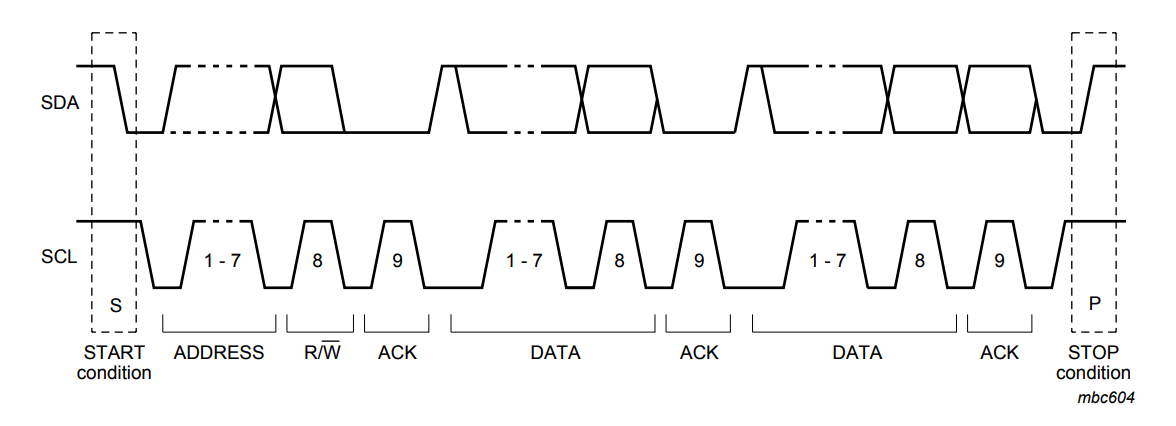
\includegraphics[width=.9\textwidth] {img/i2c-frame.png}
	\caption[I2C message diagram]{\label{fig:i2c-frame}An I2C message diagram. The frame starts with a start condition and stops with a stop condition, defined by an SDA edge while SCL is high. The address and data bytes are acknowledged by the slave by sending a 0 on the open-drain SDA line in the following clock cycle. A slave can terminate the transaction by sending 1 in place of the acknowledge bit. (\textit{Diagram taken from the I2C specification UM10204 by NXP Semiconductors})}
\end{figure}

The bus supports multi-master operation, which leads to the problem of collisions. Multi-master capable devices must implement a bus arbitration scheme as specified by the I2C standard. This feature is not often used in intelligent sensors and modules; the most common topology is multi-drop single-master, similar to SPI, with the advantage of using only two pins on the microcontroller.

\subsection{Examples of Devices Using I2C}

\begin{itemize}
	\item \textbf{APDS-9960} - ambient light, proximity and gesture sensor
	\item \textbf{L3GD20}, \textbf{BMP280}, \textbf{BME680} - listed as SPI devices, those also support I2C
	\item \textbf{DS1307} - RTC; I2C is not mentioned in the entire datasheet, presumably to avoid paying license fees, but it is fully compatible
	\item \textbf{IS31FL3730} - LED matrix driver
	\item Cameras with an SCCB port can be accessed through I2C
\end{itemize}

\section{1-Wire} \label{sec:theory-1wire}

The 1-Wire bus, developed by Dallas Semiconductor, uses a single bi-directional data line which can also power the slave devices, reducing the number of required wires to just two (compare with 3 in I2C and 5 in SPI, all including GND). 

1-Wire is open-drain and the communication consists of short pulses sent by the master and (for bit reading) the line continuing to be held low by the slave. The pulse timing (fig. \ref{fig:1w-pulses}) defines if it's a read or write operation and what bit value it carries. A transaction is started by a 480us long "reset" pulse send by master and ended by a 1-byte CRC checksum.

\begin{figure}
	\centering
	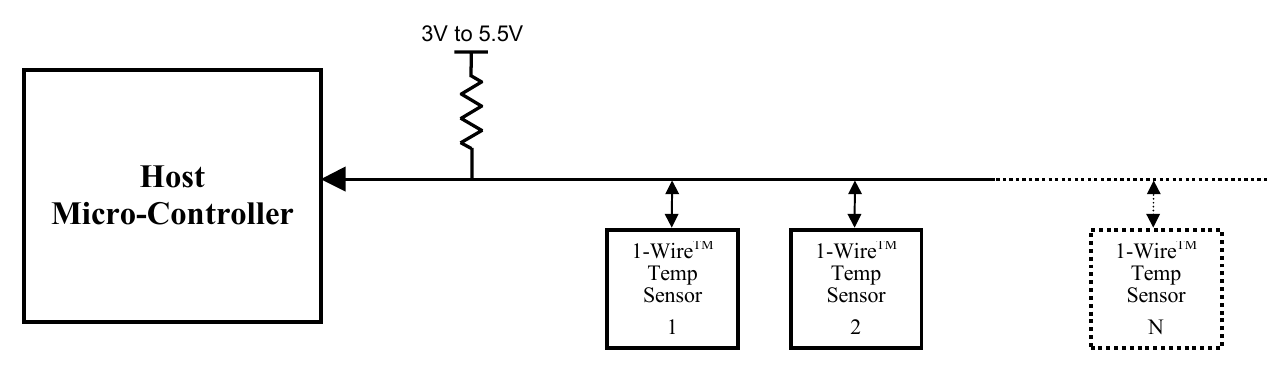
\includegraphics[width=.9\textwidth] {img/1w-topology.png}
	\caption{\label{fig:1w-topology}1-Wire topology (by \textit{Dallas Semiconductor})}
\end{figure}

1-Wire is a master-slave multi-drop bus. Devices are addressed by their unique 64-bit ID numbers (called ROMs); those IDs are found by the bus master with the cooperation from slaves using a ROM search protocol. If only one device is connected, a special command set can be used to skip addressing.

\subsection{Examples of Devices Using 1-Wire}

\begin{itemize}
	\item \textbf{DS1820}, \textbf{DS18S20}, \textbf{DS18B20} - digital thermometers
	\item \textbf{iButton} - contact-read access tokens, temperature loggers etc.
\end{itemize}

Since 1-Wire is a proprietary protocol, there is a much smaller choice of available devices and they also tend to be more expensive. The DS18x20 thermometers are, however, popular enough to warrant the bus's inclusion in GEX.

\begin{figure}
	\centering
	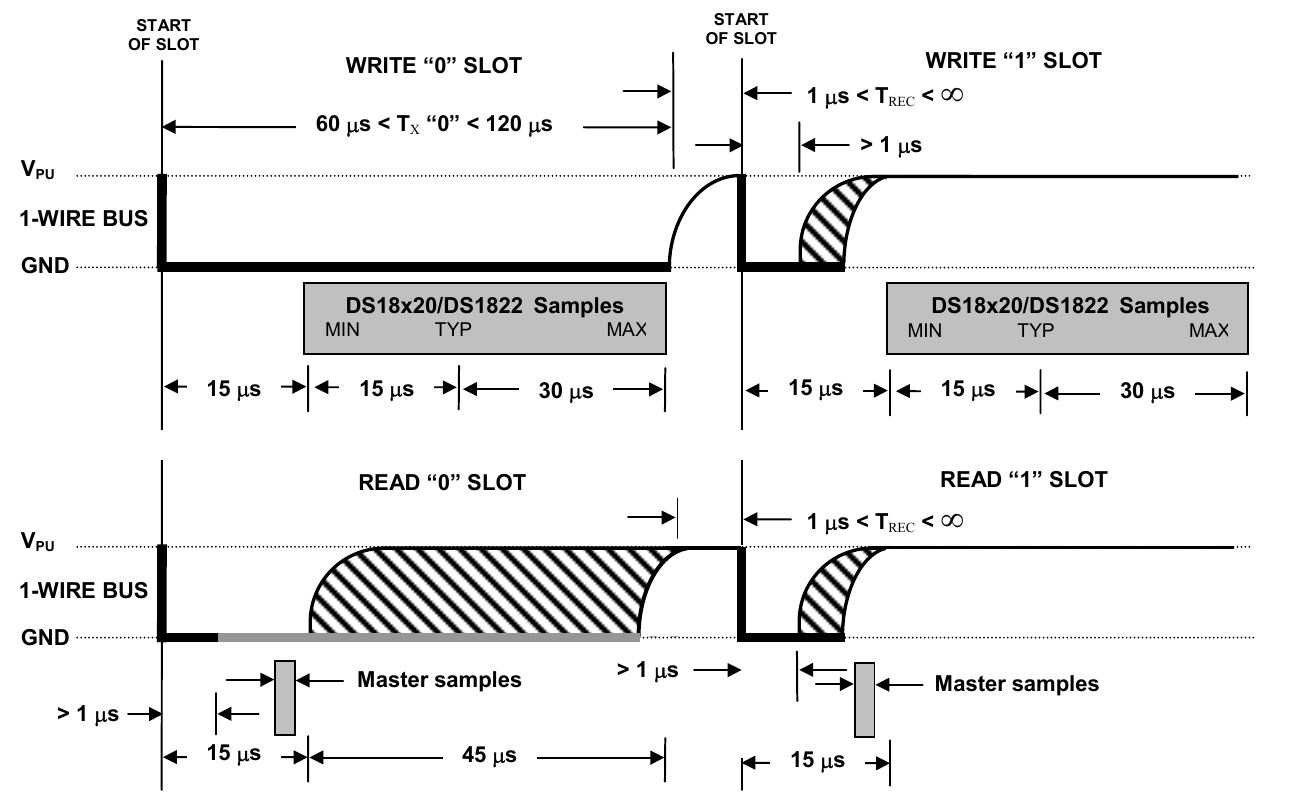
\includegraphics[width=.85\textwidth] {img/1w-rw.png}
	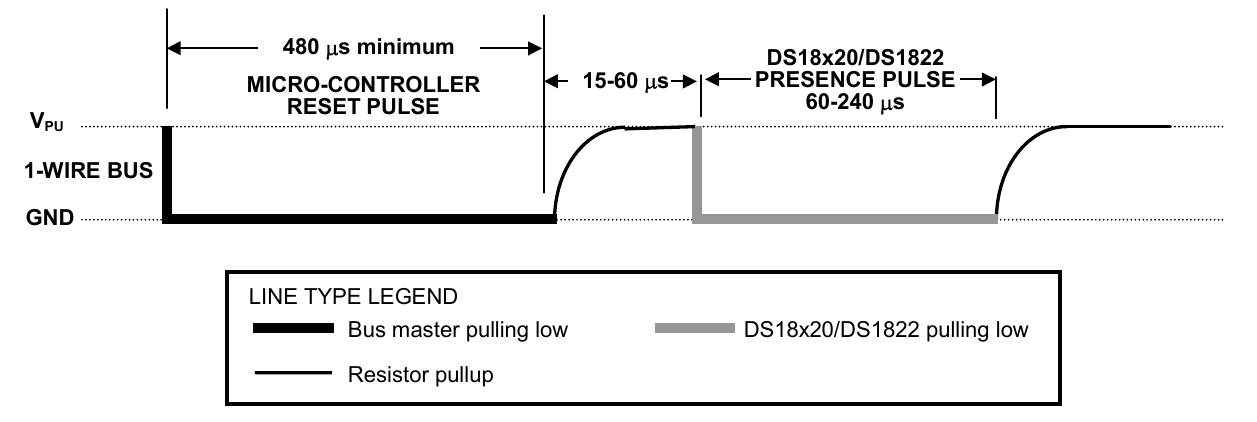
\includegraphics[width=.85\textwidth] {img/1w-reset.png}
	\caption{\label{fig:1w-pulses}The 1-Wire DIO pulse timing (by \textit{Dallas Semiconductor})}
\end{figure}

\section{NeoPixel} \label{sec:theory-neo}

NeoPixel is a marketing name of the \textbf{WS2811}, \textbf{WS2812} and compatible intelligent LED drivers that is commonly used in "addressable LED strips". Those chips include the control logic, PWM drivers and usually the LED diodes all in one miniature package.

The NeoPixel protocol is unidirectional, using only one data pin. The LED drivers are chained together. Ones and zeros are encoded by a pulse length on the data pin; after loading the color data to the LED string, a longer "reset" pulse is issued by the bus master and the set colors are displayed. The timing diagram and constraints are shown in figure \ref{fig:ws2812-dia}.

The NeoPixel timing is very sensitive to pulse length accuracy. Reliable ways to implement it use DMA with a hardware timer, or a I2S peripheral. An easier method that does not use any additional hardware resources is implementing the protocol as delay loops in the firmware; care must be taken to disable interrupts in the sensitive parts of the timing.

\begin{figure}
	\centering
	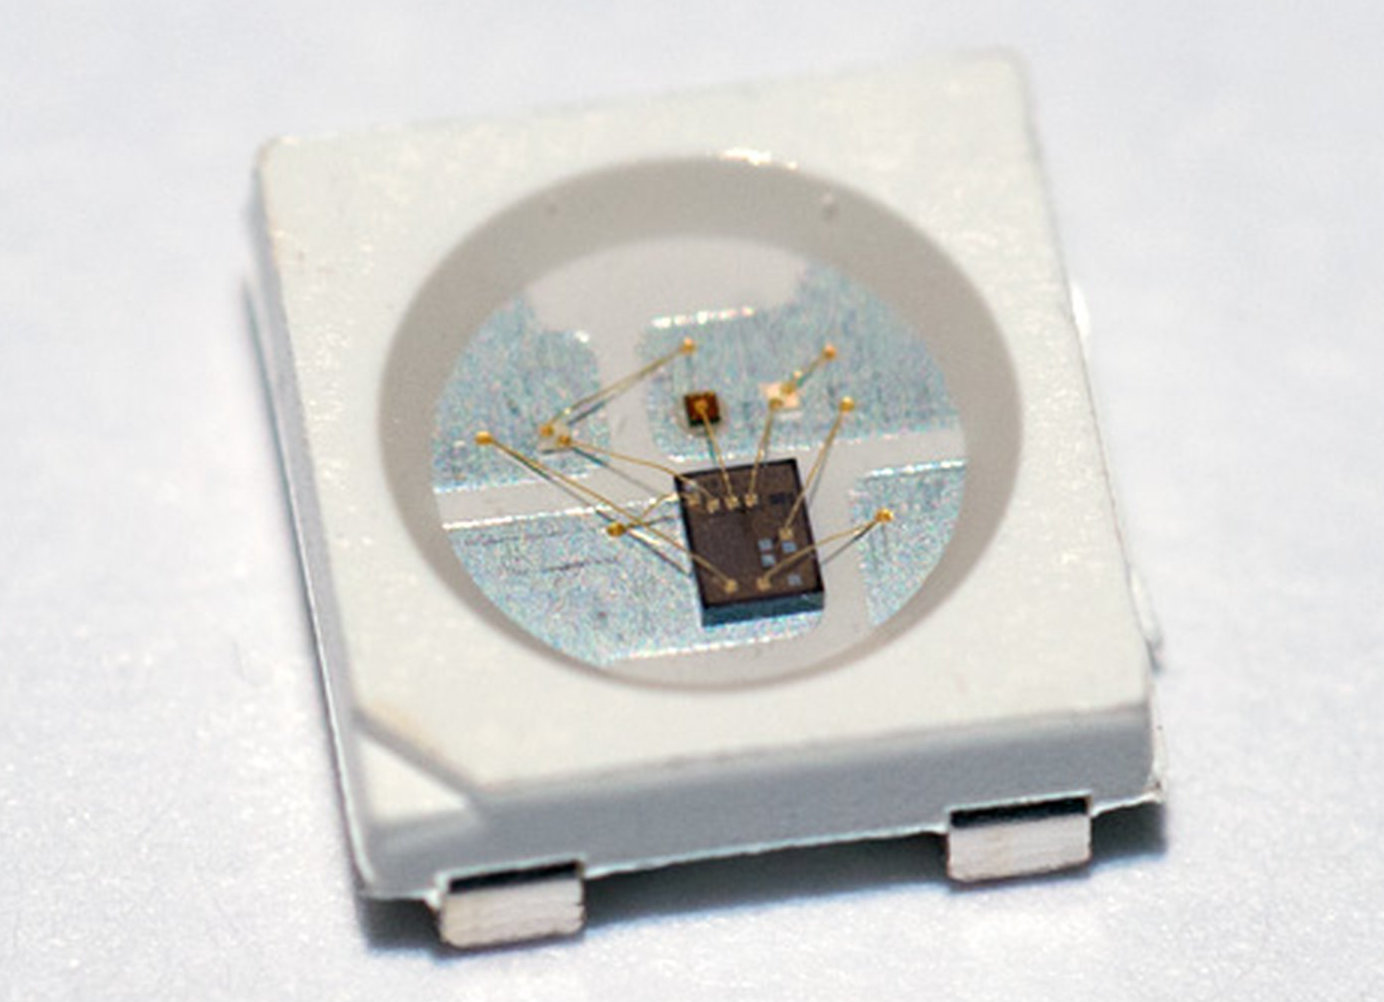
\includegraphics[width=.6\textwidth] {img/ws2812b-detail.jpg}
	\caption{\label{fig:ws2812-detail}A close-up photo of the WS2812B package, showing the LED driver IC}
\end{figure}

\begin{figure}
	\centering
	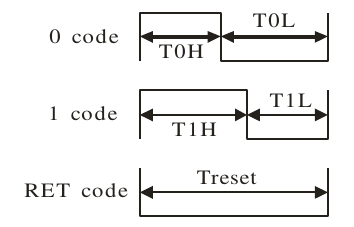
\includegraphics[width=.4\textwidth] {img/neo-diagram.png}
	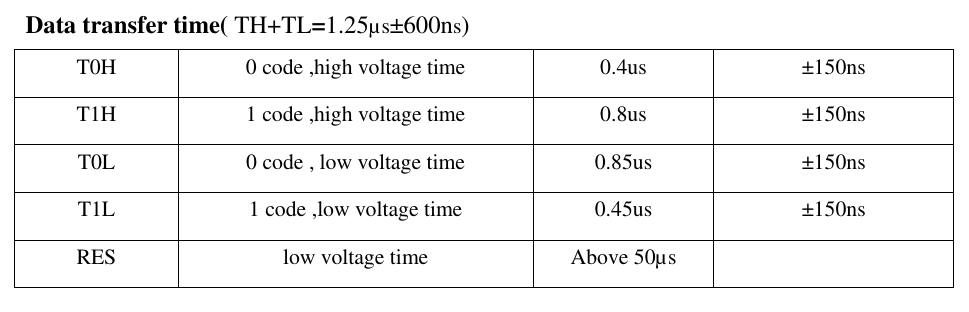
\includegraphics[width=\textwidth] {img/neo-lengths.png}
	\caption{\label{fig:ws2812-dia}NeoPixel pulse timing diagram and time constraints table \textit{(WS2812 datasheet)}}
\end{figure}
